
\chapter{Quantitative analysis reveals epidermis-specific gene module: Evidence of T-cell reprogramming in GVHD target tissues?} % Main chapter title

\label{Chapter5} % For referencing the chapter elsewhere, use \ref{Chapter1} 

%----------------------------------------------------------------------------------------

\section{Overview}

In this Chapter we utilise our module-based refined testing protocol to survey the relative expression of the 31 WGCNA-derived MataHari gene modules in both the dermis and epidermis in the presence or absence of LCs. In this way we hoped to identify any modules which were both significantly associated with, and differentially expressed in, either the dermis or epidermis as well as evaluate how results obtained using our refined testing protocol compared to those produced by a more standard methodology, the Fisher's Exact Test. 

\section{Background - Depletion of Langerhans cells (LC) in the MataHari (Female $\to$ Male) model}

As mentioned in Chapter \ref{Chapter2}, once effector T cells have been activated and recruited to a specific tissue they will interact with various resident APC populations. In the skin this includes epidermal Langerhans cells (LC). It has been demonstrated that epidermal LCs are able to exert control over T cell activation ~\autocite{Igy2013} but whether they play an additional role in the pathogenic re-programming of effector T cells within tissues is currently unclear. If it was found that interactions between CD8$\textsuperscript{+}$ T cells and tissue resident LC populations did result in re-programming of the former population, this could help further our understanding of the specific events that culminate in target organ pathology in GVHD. 

To investigate the relationship between effector T cells and epidermal LCs we adapted our MataHari F $\to$ M BMT model to allow exploration of whether interaction with resident LCs was responsible for effector CD8$\textsuperscript{+}$ T cell reprogramming, particularly for inducing the epidermis-specific gene module, M28 that was identified during previous work with this GVHD mouse model (details in Chapter \ref{Chapter1}). Using Multi-photon imaging it was shown that seven days after BMT effector T cells migrating to the skin formed connections with radio-resistant, host-derived LCs in the epidermis, but no interactions with donor-derived cells were observed most probably due to low cell counts at this time point ~\autocite{Santos}. Depletion of host-derived LCs with diphtheria toxin ~\autocite{Ben2005,Kis2005} prior to BMT revealed that this population was required for the accumulation of effector T cells in the epidermis while the depletion of host-type dermal Langerin$+$ DCs had no effect ~\autocite{Santos}. A similar requirement for LCs in the process of CD8$\textsuperscript{+}$ T cell migration into the epidermis was also seen in the B6 into 129sv model. Although LCs are known to be highly motile ~\autocite{Kis2005}, experiments depleting LCs unilaterally in one ear of a mouse at the time of BMT resulted in loss of effector T cell populations in the manipulated ear only ~\autocite{Santos}. This finding supports the notion of the need for LCs \textit{in situ}. Interestingly, host-strain LC purified from allogeneic recipients compared to those undergoing syngeneic BMT showed high levels of enrichment for IFN-g-responsive genes. It is this group of genes that are also prevalent in the gene module M28 identified using the MataHari dataset. Additionally, when host IFN-$\gamma$ receptor signalling was blocked, LCs post allogeneic BMT failed to up-regulate MHC class I expression and CD8$\textsuperscript{+}$ T cell accumulation was reduced specifically in the epidermis but not within other tissues ~\autocite{Santos}.

\section{Analysis of MataHari WGCNA-derived gene modules with standard categorical association testing method} 

Having demonstrated a requirement for LCs in the successful migration and accumulation of effector T cells in the epidermal skin compartment, we hypothesised that any gene modules involved in establishment of an inflammatory environment should be highlighted by differential expression analysis of LC depleted versus LC replete populations. To investigate this theory we surveyed the relative expression of the 31 WGCNA-derived MataHari gene modules in both the dermis and epidermis in the presence or absence of LCs (using data from the LC depletion experiments mentioned in the previous section). For each of the differential expression datasets (dermal and epidermal) we applied both a standard Fisher's Exact Test as well as our module-based refined testing protocol. For any given gene module, by plotting the differential expression \textit{p}-value against the trait association \textit{p}-value obtained as part of the WGCNA analysis (Chapter \ref{Chapter3}) we hoped to identify any modules which were both significantly associated with, and differentially expressed in, the particular skin compartment being analysed. In the following sections we present the results of this analysis, focusing initially on data from effector T cells in the dermis and then turning to the epidermal population. Both association testing methodologies are described in detail in Chapter \ref{Chapter3}. 

\subsection{Analysis of dermal effector T cell populations} 

Figures 5.1 and 5.2 below plot the results of comparing the dermis WGCNA trait association \textit{p}-value for each module (the same values apply in both comparisons) against the differential expression \textit{p}-value obtained with Fisher's Exact Test and our own module-based refined test respectively. As can be seen from both plots, the MataHari modules do exhibit varying trait associations with the dermis which is unsurprising given the variety of functions there contain as a group (see Figure 1.5), but none are particularly strong statistically. When Fisher's Exact Test was applied to quantify the extent of modular differential expression changes following LC depletion, none of the gene modules were found to be significant. This would suggest that none of the MataHari modules contain substantially more genes differentially expressed in LC depleted versus control mice than any other. Turning to the results acquired when using our refined testing protocol to analyse the differential expression data from the LC depletion study (Figure 5.2), it is evident that we do indeed see enhanced significance of certain gene modules when overall direction of effect in terms of the up-/down-regulation of module genes is incorporated into the association testing methodology (for details see Chapter \ref{Chapter3}.2.3). Examination of Figure 5.3 reveals that three of the MataHari modules, namely M4, M17 and M23, show particularly enhanced association with the dermis in LC depleted mice compared to the values seen in Figure 5.1 when using Fisher's Exact Test in isolation. 

\begin{figure}[H] 
    \centering
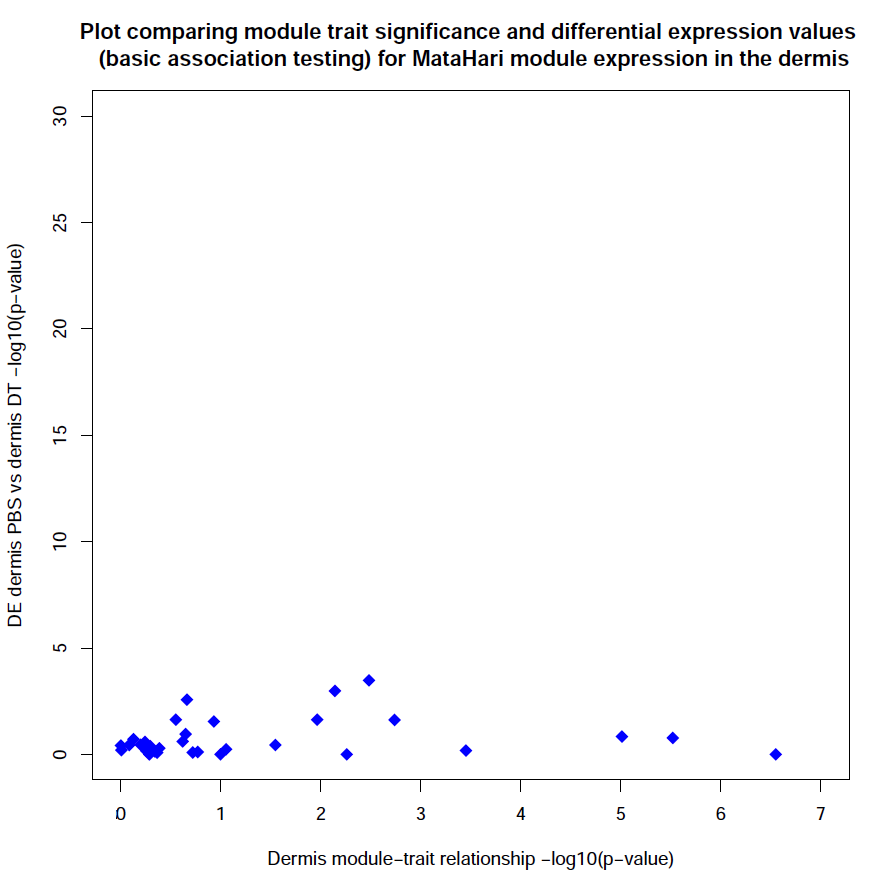
\includegraphics[width=0.6\textwidth]{Figures/Chapter5/Dermis_trait_vs_DE_BASIC.png}
\caption{\small{Graph of WGCNA-defined MataHari modules showing \textit{p}-values for correlation to dermis (x-axis) and differential expression association according to presence or absence of LC and quantified using Fisher's Exact Test (y-axis).} }
    \label{fig:23}
\end{figure}


\begin{figure}[H] 
    \centering
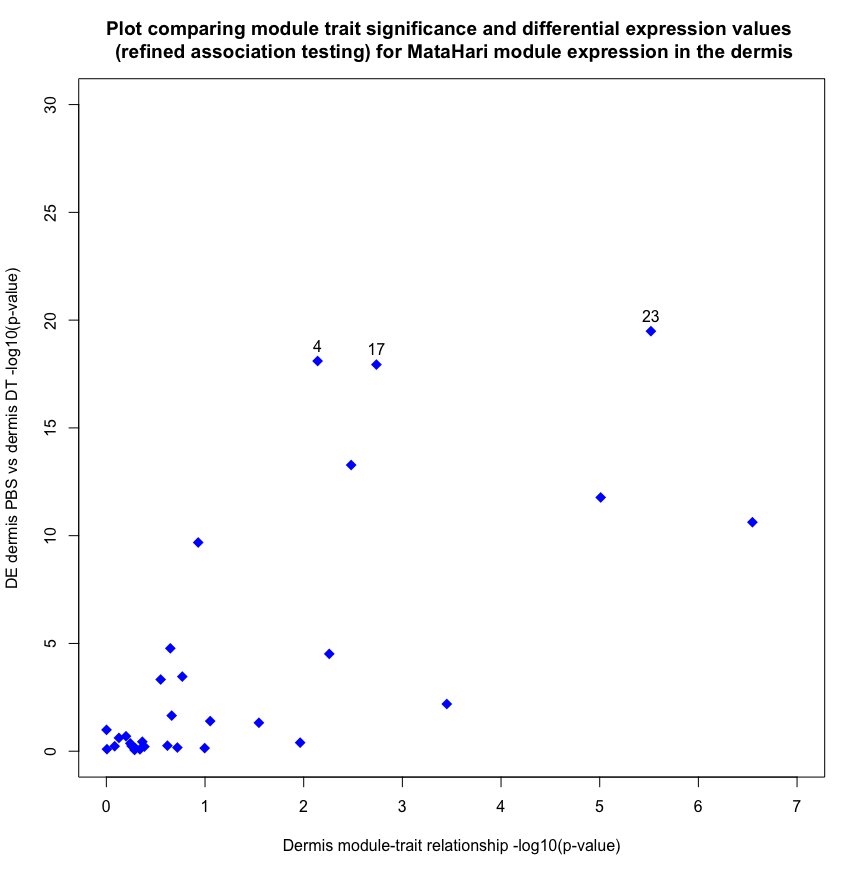
\includegraphics[width=0.6\textwidth]{Figures/Chapter5/Dermis_trait_vs_DE.png}
\caption{\small{Graph of WGCNA-defined MataHari modules showing \textit{p}-values for correlation to dermis (x-axis) and differential expression association according to presence or absence of LC and quantified using module-based refined test (y-axis).} }
    \label{fig:24}
\end{figure}

During previous work in the laboratory module based enrichment in Gene Ontology annotations were determined (Chapter \ref{Chapter3} for brief overview of WGCNA methodology) and these are summarised in Figure 1.5. Studying the annotations for M4, M17 and M23 the results are quite interesting when taken in the context of GVHD pathology. Module M4 represents a large collection of genes, many of which are involved in the key metabolic pathway responsible for ATP generation, oxidative phosphorylation ~\autocite{Santos}. The somewhat smaller gene module M17 is thought to be driven by genes encoding multiple Toll-like receptors which are known to play a key role in pathogen recognition and activation of innate immunity via the pathogen-associated molecular patterns (PAMPs) that are expressed on infectious agents ~\autocite{Santos}. These receptors also mediate the production of cytokines required for the development of effective immunity. Interestingly, the third gene module to show both significant differential expression and trait association with the dermis, M23, is comprised of many cytokine and cytokine receptor encoding genes ~\autocite{Santos}. As discussed in Chapter \ref{Chapter2}, cytokines modulate the balance between humoral and cell-based immune responses, and help regulate the maturation, proliferation and responsiveness of T cell populations. As summarised in Figure 1.5, expression of M17 and M23 was found to be enriched in the secondary lymphoid organs of allogeneic BMT recipients, while M23 was instead correlated with GVHD target organs in the same allogeneic recipient group ~\autocite{Santos}. Put together, these results indicate groups of differentially expressed genes showing association with the dermal skin compartment, in part highlighted through use of our refined testing protocol, that are known to be involved in modulating immune responses and cytokine activity. Thus by utilising modular direction of effect data we can enhance the sensitivity of differential expression based analysis, in this case highlighting changes in expression levels of inflammatory related genes when LCs are depleted in the dermis. 

\subsection{Analysis of epidermal effector T cell populations} 

Applying the same differential expression analyses in combination with WGCNA derived trait associations to epidermal data, we obtain the module association results depicted in Figures 5.3 and 5.4 below. 

\begin{figure}[H] 
    \centering
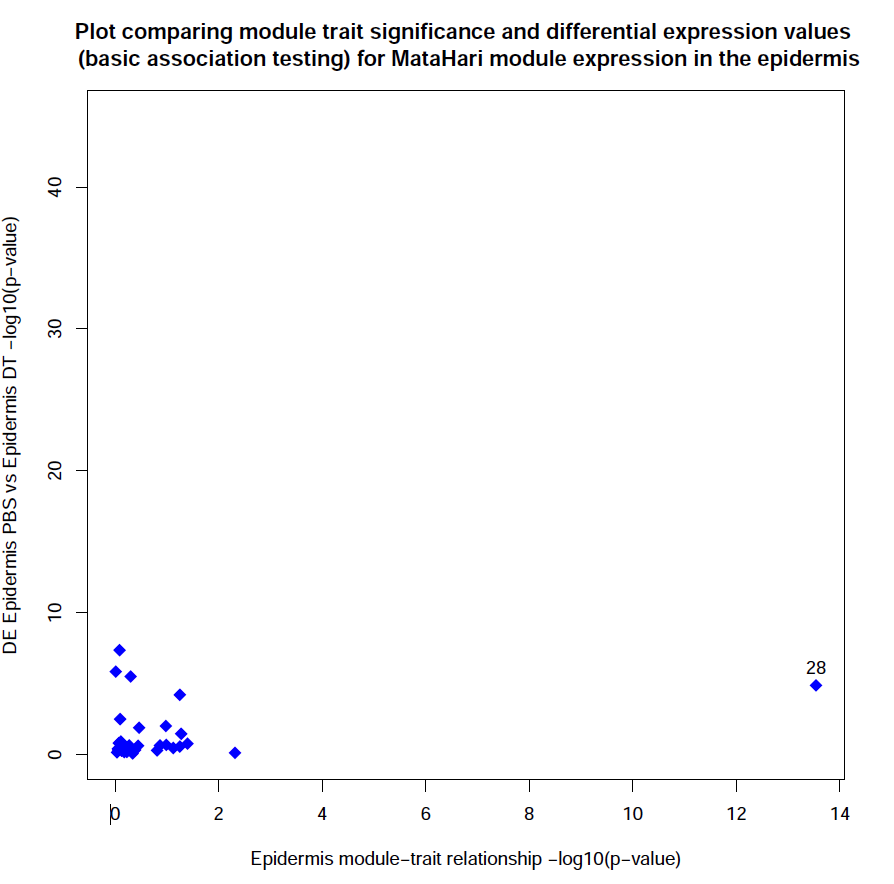
\includegraphics[width=0.5\textwidth]{Figures/Chapter5/Epidermis_trait_vs_DE_BASIC.png}
\caption{\small{Graph of WGCNA-defined MataHari modules showing \textit{p}-values for correlation to epidermis (x-axis) and differential expression association according to presence or absence of LC and quantified using Fisher's Exact Test (y-axis).} }
    \label{fig:25}
\end{figure}

As is clear from a comparison of Figures 5.1 and 5.3, there are notable differences between the relative significance of trait associations of the 31 MataHari gene modules in the dermis and epidermis. Whereas the modules showed a range of trait association values in the dermis data, they generally appear much more clustered at low significance values in the epidermis samples. That being said, the epidermis data reveals one marked exception, module M28. As evidenced by Figure 5.3, MataHari module M28 is strongly associated with the "dermis trait" and yet does not stand out in terms of differential expression significance. However, application of our module-based refined association test gives a very different picture. 

Figure 5.4 shows the difference made by including direction of effect data during the module association testing. Several of the MataHari modules now exhibit highly significant differential expression associations in the LC depletion dataset, with much stronger \textit{p}-values than seen in the dermis. What is more interesting however is that a substantial jump in significance is observable in the case of M28. As can be seen clearly in Figure 5.4, gene module M28 is unique in both the dermal and epidermal datasets as being significantly expressed in the epidermis and showing a very high level of differential expression in the presence or absence of LC (\textit{p}$<10^{-30}$). This effector T cell module was thus found to be highly specific for the epidermal compartment of the skin and as mentioned in Chapter \ref{Chapter1} contains genes relating to Interferon-$\gamma$ signalling including many pro-inflammatory cytokines (e.g. Ifng, Il2, Il3, Csf1 and Csf2), cytokine receptors and downstream adaptors (e.g. Il2ra, Il1r1, Il18rap) ~\autocite{Santos}.  Interferon-$\gamma$ is believed to be a primary driver gene for module M28 and follow-up experiments demonstrated the reduction of this genes mRNA and protein expression levels in LC depleted mice ~\autocite{Santos}. 

\begin{figure}[H] 
    \centering
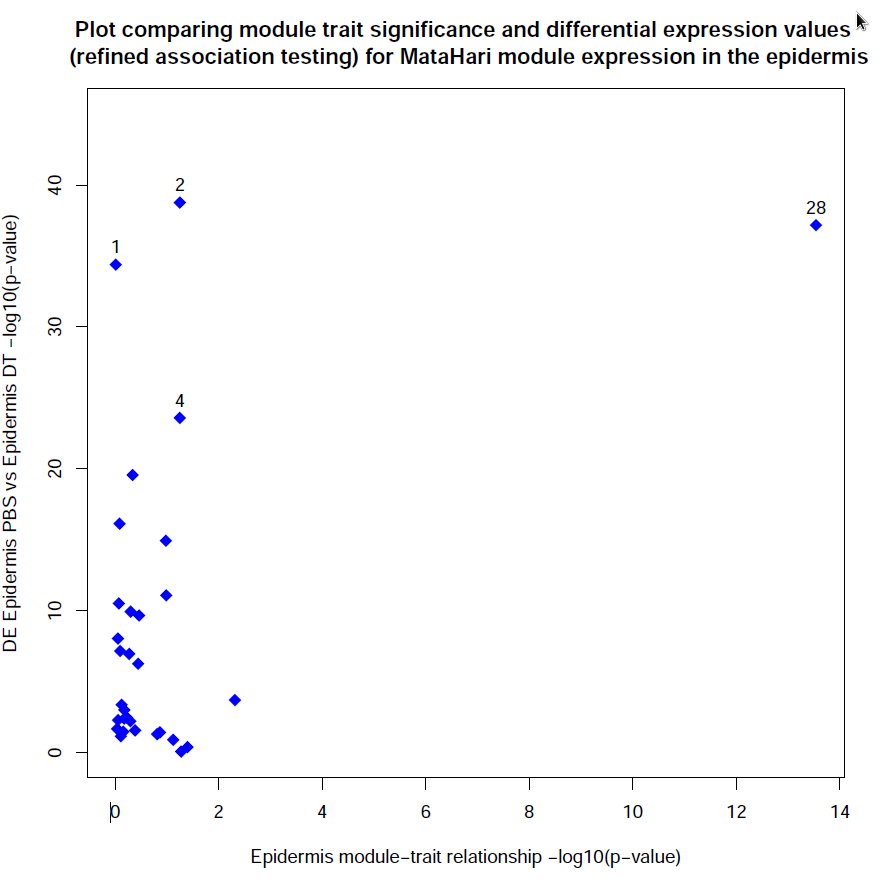
\includegraphics[width=0.6\textwidth]{Figures/Chapter5/Epidermis_trait_vs_DE.png}
    \label{fig:26}
\caption{\small{Graph of WGCNA-defined MataHari modules showing \textit{p}-values for correlation to dermis (x-axis) and differential expression association according to presence or absence of LC and quantified using module-based refined test (y-axis).} }
\end{figure}

\section{Conclusions}

When viewed as a whole, the results presented in this Chapter suggest the plausible existence of a feed-forward loop governing tissue-specific effector T cell pathogenicity in which Interferon-$\gamma$ production by effector T cells entering the epidermis up-regulates MHC I expression on LCs. This in turn, this facilitates LC-effector T cell cognate interaction, causing up-regulation of the M28 gene module, and enhanced effector T cell survival and localised cytokine production ~\autocite{Santos}. This work also emphasises the utility and potential power of the module-based refined association testing protocol developed as part of this project. It is clear from the results presented above that the increased sensitivity obtained by the incorporation or direction of effect data can reveal hidden signals in real datasets as well as simulated ones. 

